Modify Program 12 (p. 57) to make use of chebfft instead of cheb. The results should be the same as in
Output 12, except for rounding errors. Are the effects of rounding errors smaller or larger than
before?\\\\

\begin{solution}\renewcommand{\qedsymbol}{}\ \\ 
    Below are the graph outputs of program 12, the first of which is using cheb and the second using
    chebfft:

    \begin{figure}[htp]
        \centering
        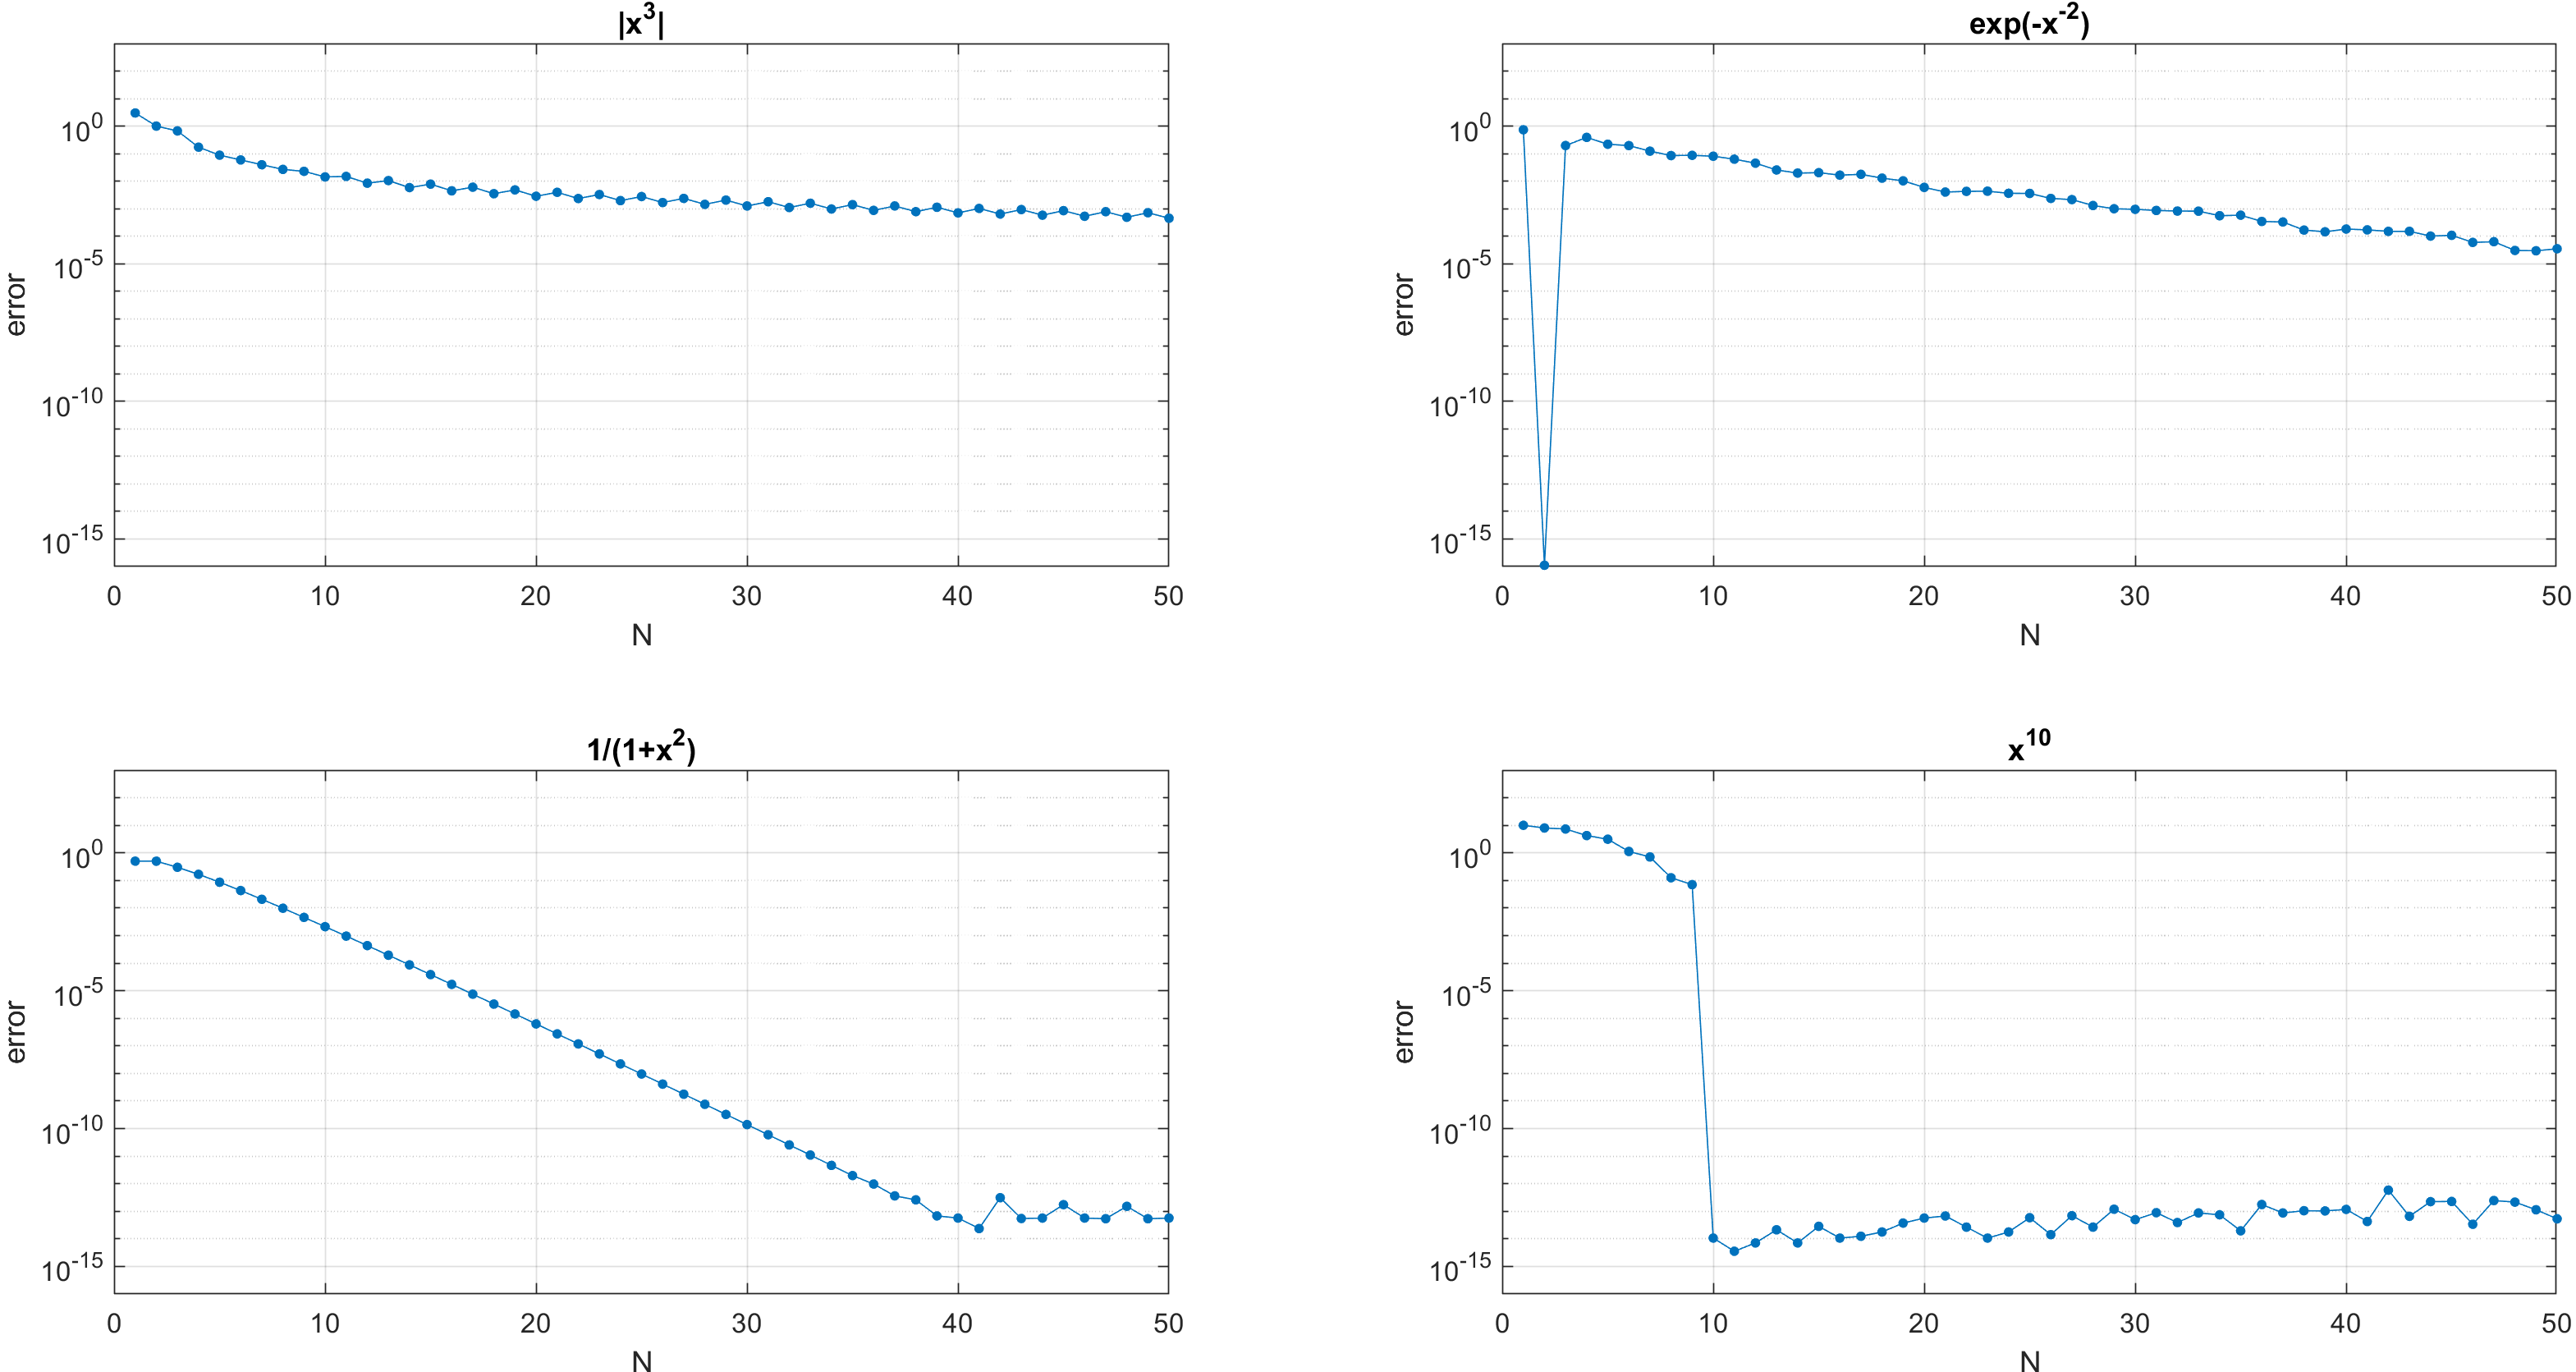
\includegraphics[scale=0.14]{8_3cheb.PNG}
        \caption{cheb}
    \end{figure}
    \begin{figure}[htp]
        \centering
        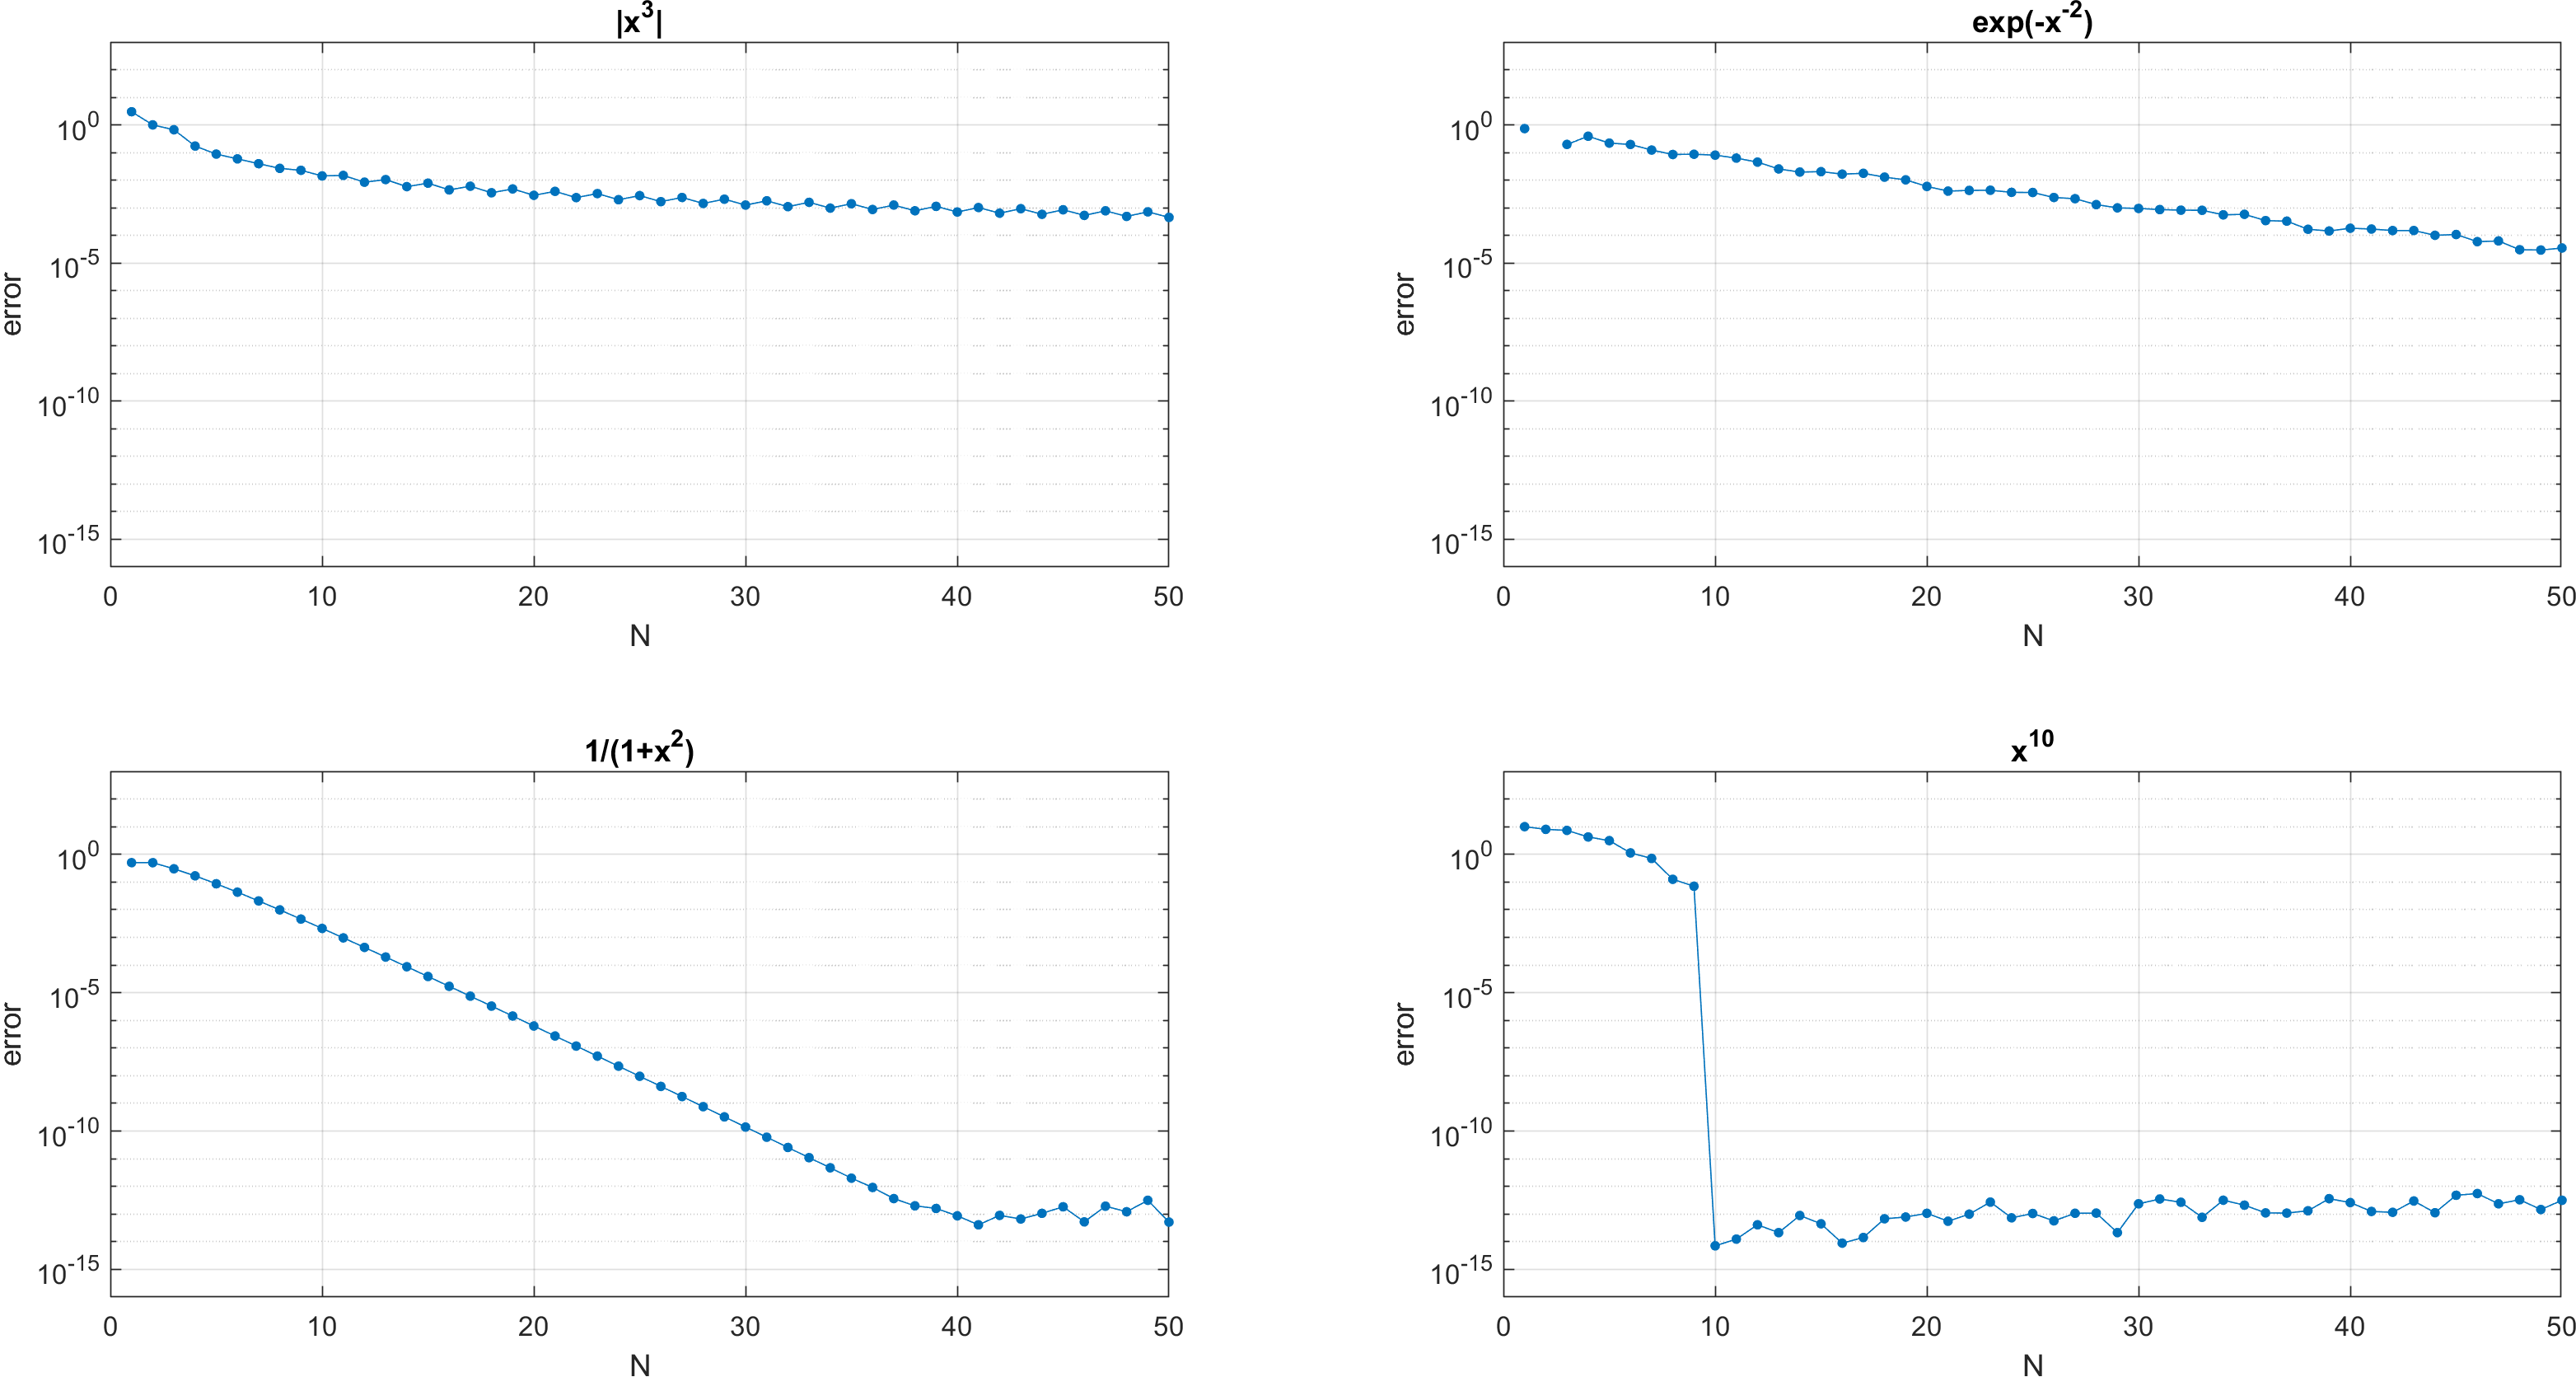
\includegraphics[scale=0.14]{8_3chebfft.PNG}
        \caption{chebfft}
    \end{figure}

    We see that the round off error is the only difference between the two graphs. It can also be seen
    that the rounding error for the chebfft function is slightly less than that of the regular cheb
    function.

\end{solution}

\newpage
\lstinputlisting{problem8_3.m}
\newpage